\begin{question}
	Let $(X_n)$ be the simple random walk on the following graph. Compute $\prob_0(T_3<T_7)$.
	
	\begin{center}
		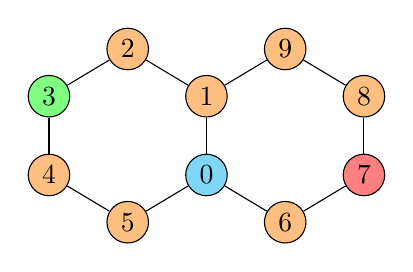
\begin{tikzpicture}[scale=1, every node/.style={circle, draw}]
			\tikzstyle{every node}=[circle, draw, fill=orange!50,
			inner sep=0pt, minimum width=15]
			
			
			\node[fill=cyan!50] (n0) at (0,0) {0};
			\node (n1) at (0,1) {1};
			\node (n2) at (-1,1.6) {2};
			\node[fill=green!50] (n3) at (-2,1) {3};
			\node (n4) at (-2,0) {4};
			\node (n5) at (-1,-0.6) {5};
			\node (n9) at (1,1.6) {9};
			\node (n8) at (2,1) {8};
			\node[fill=red!50] (n7) at (2,0) {7};
			\node (n6) at (1,-0.6) {6};

			\draw (n0) -- (n1);
			\draw (n1) -- (n2);
			\draw (n2) -- (n3);
			\draw (n3) -- (n4);
			\draw (n4) -- (n5);
			\draw (n5) -- (n0);
			\draw (n0) -- (n6);
			\draw (n6) -- (n7);
			\draw (n7) -- (n8);
			\draw (n8) -- (n9);
			\draw (n9) -- (n1);

			
		\end{tikzpicture}
	\end{center}
\end{question}
\begin{ans}
	For a much more simpler solution, let's define the two following notations
	\[ B = \{T_3 < T_7\}, \qquad p_v = \prob_v(B). \]
	Then, by first step argument at state $0$, we can write
	\[ p_0 = \frac{1}{3} (p_5 + p_6 + p_1).  \tag{5.1}\]
	Now we need to evaluate each of the terms in the right hand side. We start with $p_5$.
	\[ p_5 = \prob_5(B) = \underbrace{\prob_5(B|T_3<T_0)}_{1}\underbrace{\prob_5(T_3<T_0)}_{1/3} + \underbrace{\prob_5(B|T_3>T_0)}_{p_0}\underbrace{\prob_5(T_3>T_0)}_{2/3} = \frac{1}{3} + \frac{2}{3}p_0. \]
	note that $\prob_5(B|T_3<T_0) = 1$, since if we get to state 3, before getting to state 0, then it means that we have reached the state 3 before reaching the state 7, thus the event $B$ occurs with probability 1. Also $\prob_5(T_3<T_0) = 1/3$ from the Gambler's ruin. Furthermore $\prob_5(B|T_3>T_0) = p_0$ by using the Markov property, and finally $\prob_5(T_3>T_0) = 2/3$ by the Gambler's ruin. \\
	Now, we need to evaluate the term $p_6$. To analyze this term, we will do a first step argument starting at this point
	\[ p_6 = \prob_6(B) = \frac{1}{2}(\underbrace{p_7}_{0} + p_0) = \frac{p_0}{2}. \]
	Note that $p_7 = 0$, since then the event $B$ has not occurred. \\
	Finally, we need to analyze the term $p_1$. Again, by first step argument on this state we have
	\[ p_1 = \frac{1}{3}(p_0 + p_9 + p_2). \]	
	By doing a analysis on $p_9$ similar to the one we did for 5, we can write
	\[ p_9 = \prob_9(B)= \underbrace{\prob_9(B|T_7<T_1)}_{0}\prob_9(T_7<T_1) + \underbrace{\prob_9(B|T_7>T_1)}_{p_1}\underbrace{\prob_9(T_7>T_1)}_{2/3} = \frac{2}{3}p_1. \]
	The rationale behind the values for each term in the equation above, is exactly the same as in analyzing the terms of $p_5$.\\
	Now, we analyze the term $p_2$ by performing another first step analysis, similar to the one we did for state 6.
	\[ p_2 = \frac{1}{2}(\underbrace{p_3}_1 + p_1) = \frac{1}{2}(1+p_1). \]
	Now we can calculate $p_1$ in terms of $p_0$ which turns out to be
	\[ p_1 = \frac{6}{11}p_0 + \frac{3}{11}.  \]
	Now we insert all of the terms in the equation $(5.1)$ to get
	\begin{align*}
		&3p_0 = \frac{1}{3}+\frac{2}{3}p_0 + \frac{1}{2}p_0 + \frac{6}{11}p_0 + \frac{3}{11} \\ 
		&\implies 3p_0 - \frac{113}{66}p_0 = \frac{40}{33} \\
		&\implies p_0 = \frac{66}{85}\cdot\frac{40}{33} = \frac{16}{17}\\
		&\implies \boxed{p_0 = \frac{16}{17}}.
	\end{align*}


	\qed
	
	

\end{ans}